\chapter{Background}\label{chap:background}
Explain the math and notation.
% \begin{algorithm}[p]
\caption{Stochastic Gradient Descent: Neural Network}
\label{alg:backpropnn}
\begin{algorithmic}
    % \ttfamily
    \State Create a mini batch of $m$ samples $\vec{x}_0 \ldots \vec{x}_{m-1}$
    \ForEach{sample $\vec{x}$}
        \State $\vec{a}^{\vec{x},0} \gets \vec{x}$  \alignedComment{Set input activation}
        \ForEach{Layer $l \in \{1\ldots L-1\}$}  \alignedComment{Forward pass }
            \State $\vec{z}^{\vec{x},l} \gets \mathbf{W}^l \vec{a}^{\vec{x},l-1}+\vec{b}^l$
            \State $\vec{a}^{\vec{x},l} \gets \varphi(\vec{z}^{\vec{x},l})$
        \EndFor
        \State $\bm{\delta}^{\vec{x},L} \gets \nabla_{\vec{a}} C_\vec{x} \odot \varphi'(\vec{z}^{\vec{x},L})$ \alignedComment{Compute error}
        \ForEach{Layer $l \in L-1, L-2 \ldots 2$}  \alignedComment{Backpropagate error}
            \State $\bm{\delta}^{\vec{x},l} \gets ((\mathbf{W}^{l+1})^T \bm{\delta}^{\vec{x},l+1})\odot \varphi'(\vec{z}^{\vec{x},l})$
        \EndFor
    \EndFor
    \ForEach{$l \in L, L-1 \ldots 2$} \Comment  \alignedComment{Gradient descent}
        \State $ \mathbf{W}^l \gets \mathbf{W}^l-\frac{\eta}{m} \sum_\vec{x} \bm{\delta}^{\vec{x},l} (\vec{a}^{\vec{x},l-1})^T$
        \State $\vec{b}^l \gets \vec{b}^l-\frac{\eta}{m}\sum_\vec{x} \bm{\delta}^{\vec{x},l}$  
    \EndFor
\end{algorithmic}
\end{algorithm}
% 
%
% \begin{figure}[t]
%     \begin{center}
%     \begin{tikzpicture}
%         \node (a) at (0,0) {a};
%         \node (b) at (2, 0) {b};
%         \draw[->] (a) -- (b);
%
%
%     \end{tikzpicture}
%     \end{center}
%     \caption[Tikz Example]{Use tikz to draw nice graphs!}
%     \label{fig:Tikz}
% \end{figure}


\todo{Add section about DNA?}
% \section{Deoxyribonucleic acid}\label{sec:dna}

\section{Chromosome Conformation Capture and Hi-C}\label{sec:c3}\label{sec:hic}

\begin{figure}[t]
\begin{centering}
%    \subfloat[Diagram summarising the Hi-C experimental protocol. The red and blue rectangles represent cross-linked restriction fragments while the yellow marker shows the position of biotin incorporation.]
%    \subfloat[Generation of the Hi-C ligation junction sequence by successive digestion (with HindIII in this example), fill in and blunt-ended ligation steps. The modified restriction site sequence is not found in the original genomic sequence.]
    {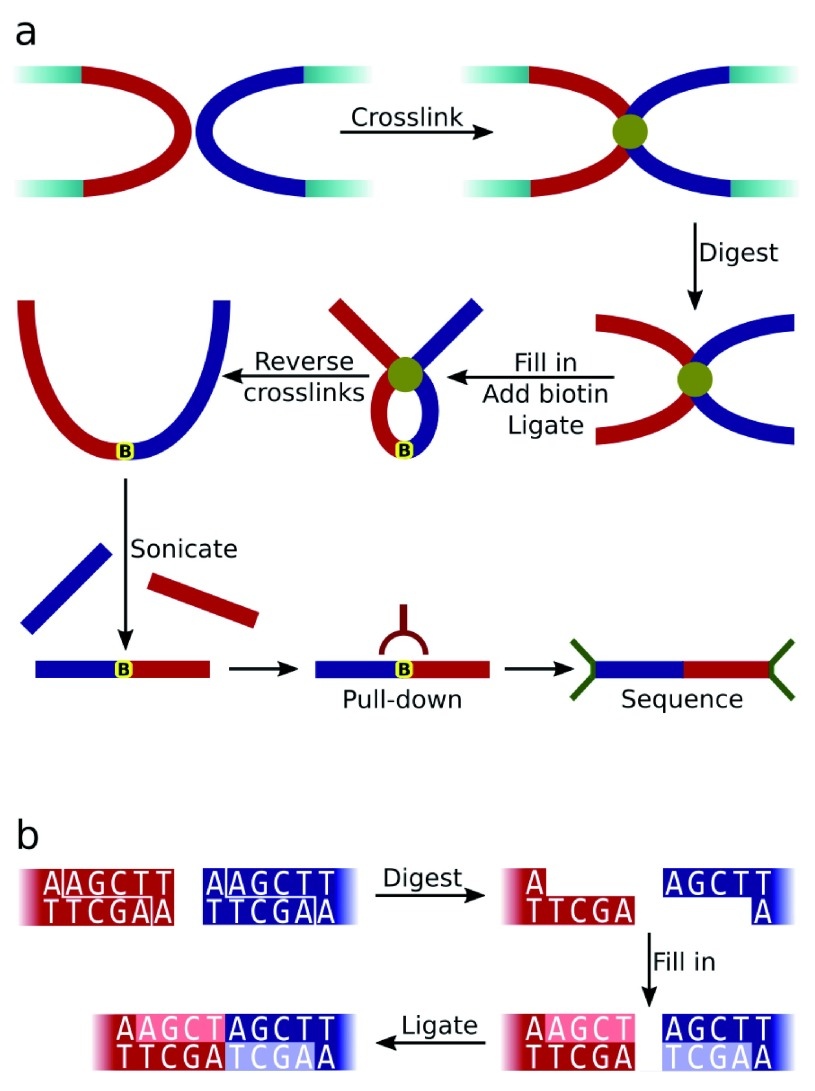
\includegraphics[scale=4]{figures/background/f1000research-4-7903-g0000.jpg}}
    \caption[Summarised Hi-C protocol]
    {\textbf{a)} Diagram summarising the Hi-C experimental protocol. The red and blue rectangles represent cross-linked restriction fragments while the yellow marker shows the position of biotin incorporation. \textbf{b)} Generation of the Hi-C ligation junction sequence by successive digestion (with HindIII in this example), fill in and blunt-ended ligation steps. The modified restriction site sequence is not found in the original genomic sequence. \\ \\ Image and description taken from \cite{wingett2015hicup}.}
    \label{fig:HiC}
    \todo{rewrite the description in my own words}

    \todo{remove the b section}
\end{centering}
\end{figure}



    % {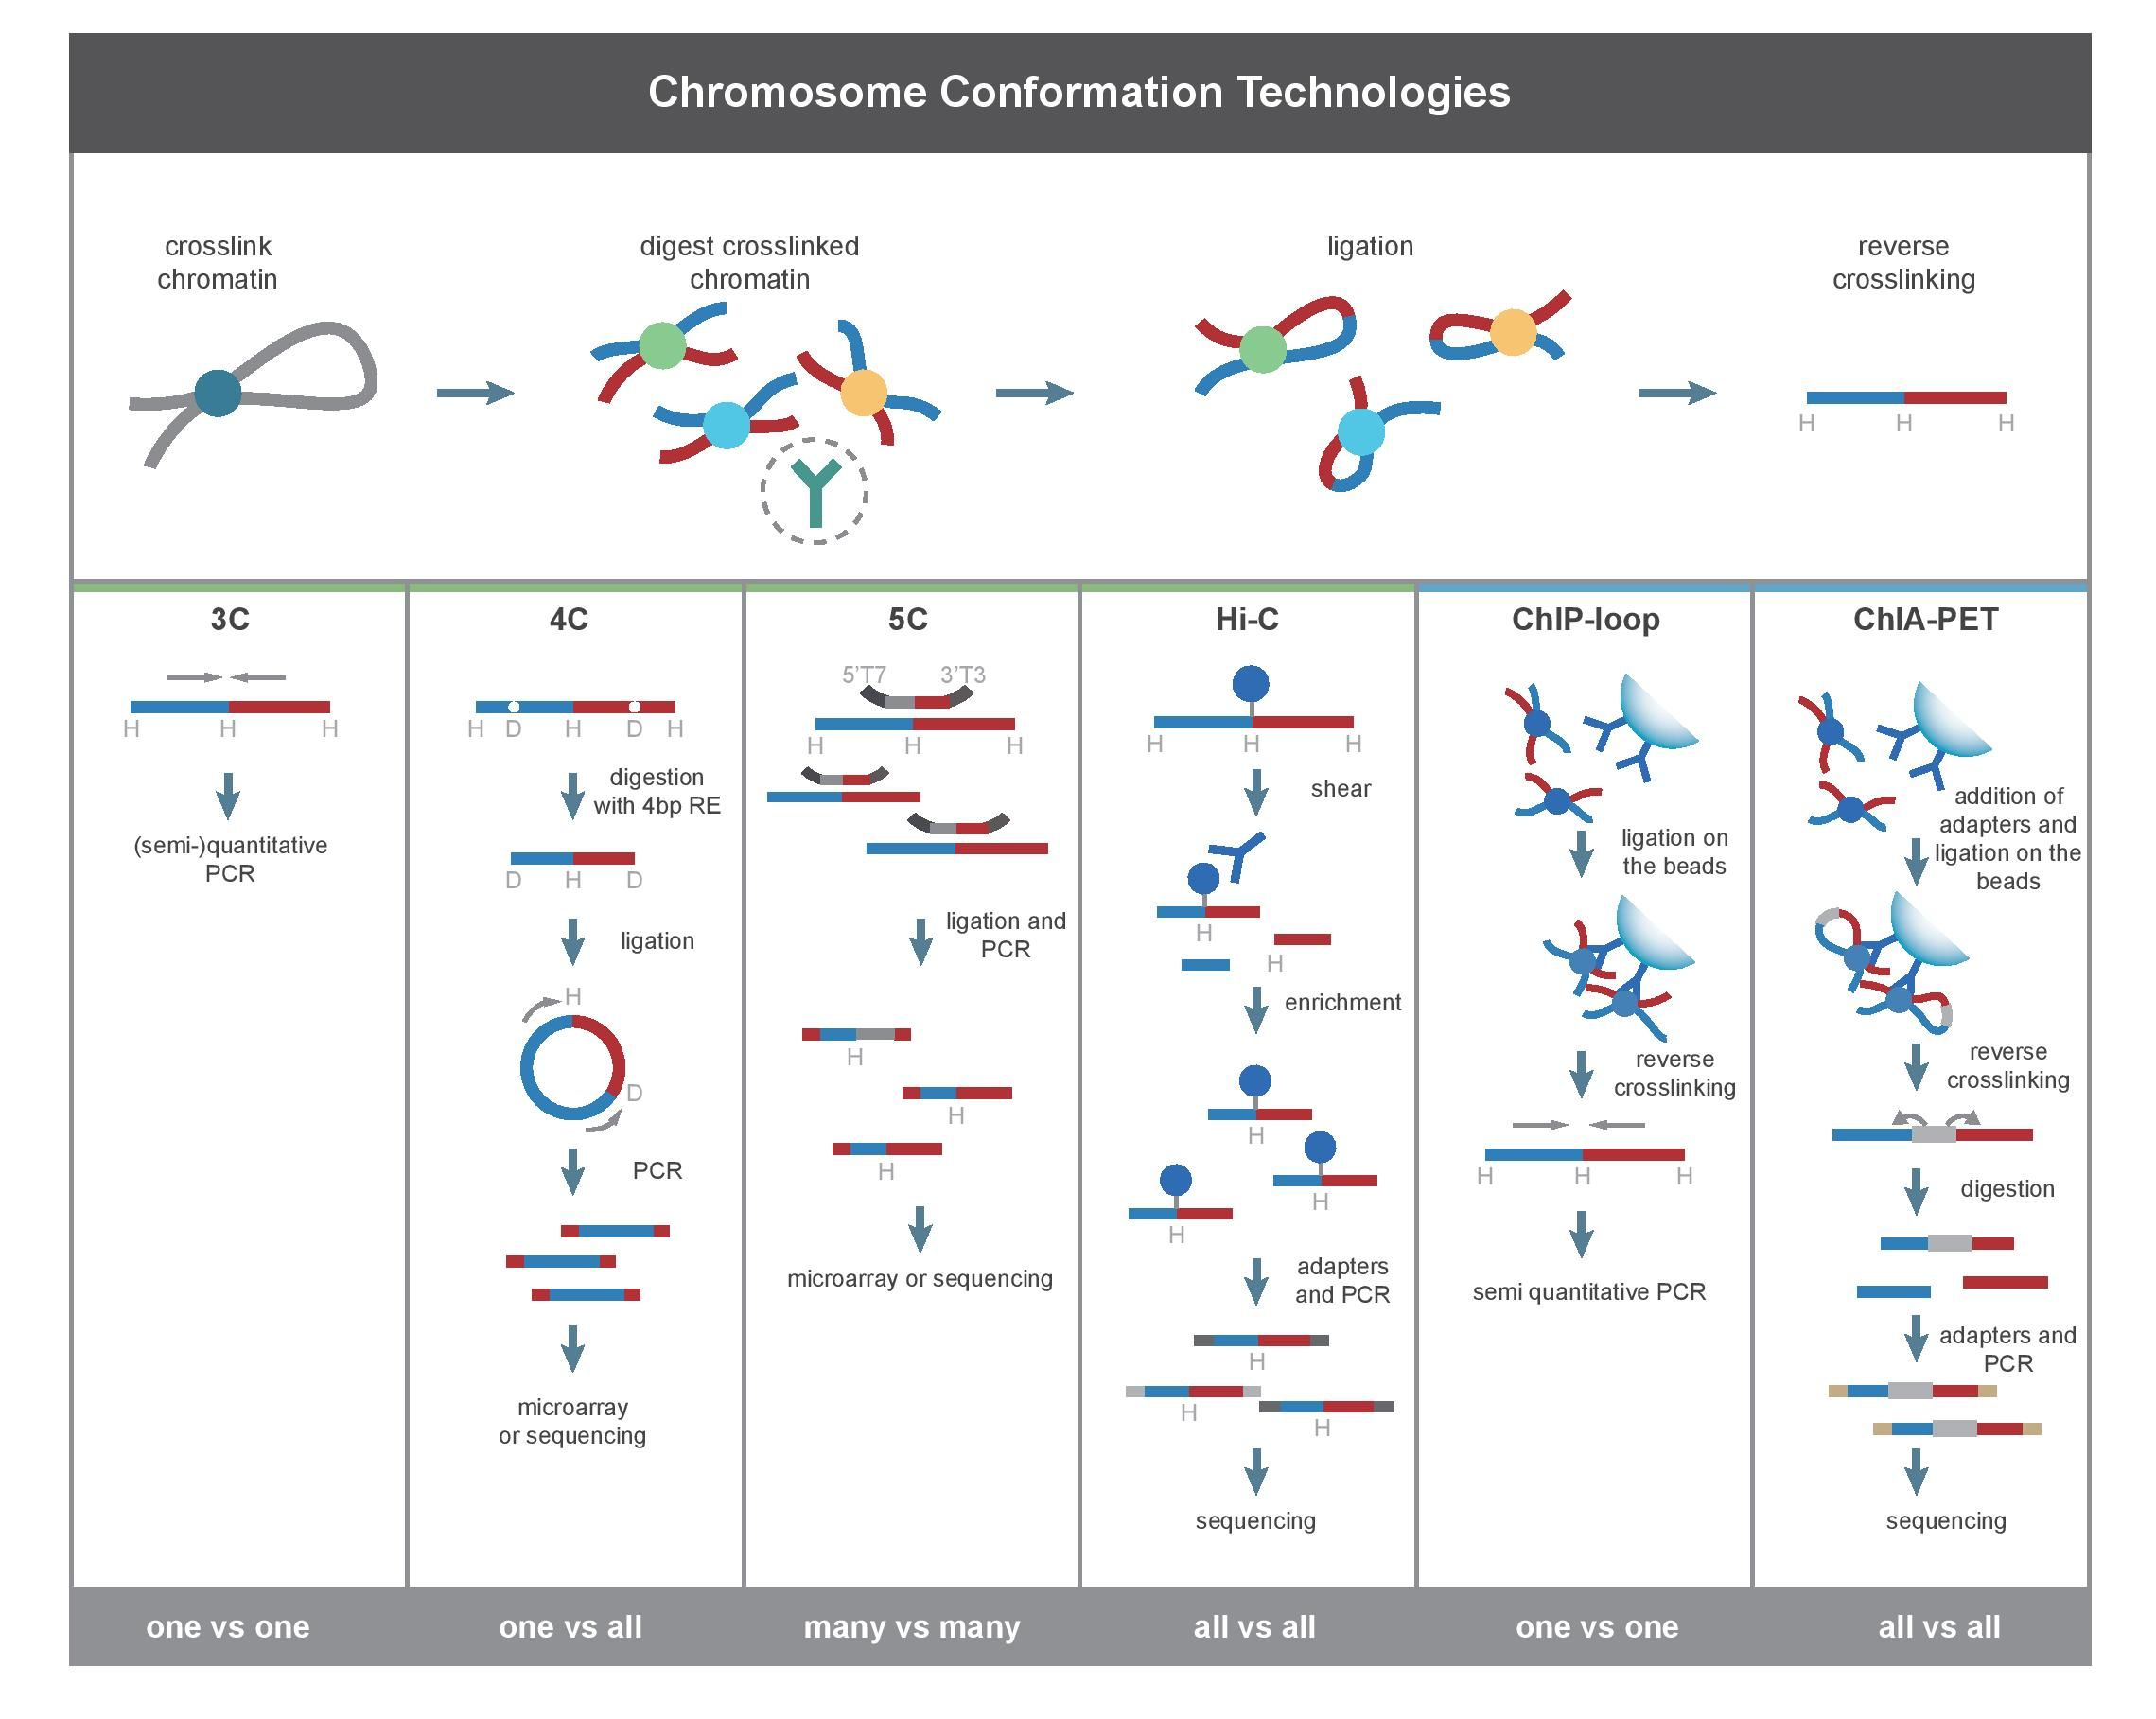
\includegraphics[scale=0.8]{figures/background/Chromosome_conformation_techniques.jpg}}
    % \caption[Comparison among 3C and its derived methods]{\textbf{Comparison among 3C and its derived methods} Source: https://en.wikipedia.org/wiki/File:Chromosome\_conformation\_techniques.jpg}


\subsection{Overview}


Chromatin usually describes different levels of how DNA organizes itself. The
well-known double-helix is only the lowest of several structural layers.

Looking at it from the outside (highest structural layer), DNA seems to be kind
of like a big ball of wool. With the help of Hi-C (and similar methods) we can
visualize spacial proximity. Regulating \draft{correct wording?} genes also
have effect on their spatial neighbourhood, not only on the neighbourhood
going up and down the strand of DNA.



Chromosome Conformation Technologies describe several similar methods to
compare genomic loci. They all start by:

\begin{itemize}
    \item creating chromatin cross-links
    \item digesting the cross-linked chromatin and
    \item ligating the ends
\end{itemize}

to get a reversed cross-link sequence.

\subsection{Cross-linking DNA}

The first step, as shown in \figref{fig:HiC} is to cross-link DNA strands that
are close to each other spatially. This is done by adding formaldehyde, which
bonds sufficiently close strands together.

A chromatin cross-link is two entirely different parts of the genome held
together by a chemical bond with formaldehyde. This process cannot be
specifically controlled, so only 'regions near each other' are connected, not
necessarily two 'known to be close' regions.

\subsection{Digestion}

The next step is cutting the whole ball of wool apart in certain intervals. For
this, restriction-enzymes are used (specifically restriction endonuclease).
Commonly used enzyme here would be EcoR1 or HindIII \todo{add reference or
sth}, cutting the genome about every 4000 base-pairs.

This is cutting the whole genome apart, leaving some (cross-) linked and some unlinked parts.

\subsection{Ligation}

Next, we randomly ligate (connect together) ends which we previously cut apart.
This is done using biotin \todo{more details!}.
Some of the reconnected will have been together before as well, so this is
usually done in less concentrated environments. The goal here is to get the
previously linked parts to be connected.

\subsection{Reverse Cross-links}

\extend{This}
As soon as the formaldehyde is removed, reverse cross-links remain.
\todo{where does the name come from / what does it mean} 
\todo{How is the formaldehyde removed}

\subsection{Sonication}

\todo{actually write this.}
% - they are being sonicated with certain frequencies, so that they break apart
%   in shorter fragments
% - question: is biotin a shock-absorbar, which is why it's not breaking at these points?

\subsection{Removal of biotin}

\todo{actually write this.}
% - called pull down
% - removal of biotin

\subsection{Sequencing}

\todo{actually write this.}
% - putting the 3' and 5' ends there
% - usual PCR methods


% Open questions:
% - scaffolds?

% Chromatin is packaged into three-dimensional structures, that retain a
% relationship between genomic and physical distance. Sequences that are closer
% on the same chromosome, are also closer in physical space. Our method
% exploits this relationship between linkage and proximity to enable whole
% chromosomes scaffolding and phasing of genomes.
%
% The DNA in the sample is cross-linked in-vivo to fix DNA sequences present
% inside the same cell. Cross-linking trap sequence interactions across the
% entire genome and between different chromosomes.
%
% Cross-Linked DNA is fragmented with endonucleases. Fragmented loci are then
% biotin elated and ligated creating chimeric junctions between adjecent
% sequences. This process is called proximity ligation.
%
% The more often two sequences are joined together, the closer these two
% sequences are in genomic space.
%
% Biotinylated junctions are purified and subjected to paired-end sequencing.
% The proximity-ligation-reads are then mapped onto a draft assembly.
%
% Proximity information is used to assign context to chromosomes, and order and
% orient them along chromosome scale scaffolds.
%
% This results in fully scaffolded chromosomes of virtually any size. This
% process also detects structural variation and corrects assembly miss-joins as
% well as maps the three-dimensional conformation of chromatin within a
% population of cells.

% See \figref{fig:HiC}.


% Background:
\todo{Cite/introduce/... the given papers, and introduce the required concepts}

Required concepts:
\begin{itemize}
    \item Biology:
    \item Chromosome Conformation Capture
    \item Hi-C  + pipeline
    \item The iterative algorithm (again ?)
    \item analysis that can be done further
    \item outlook. Meaning: What can be done, when having the 3C-Data?
\end{itemize}





